\documentclass[12pt,letterpaper,fleqn]{article}
\usepackage{fullpage}
\usepackage[top=2cm, bottom=4.5cm, left=2.5cm, right=2.5cm]{geometry}
\usepackage{amsmath,amsthm,amsfonts,amssymb,amscd}
\usepackage[utf8]{inputenc}
\usepackage{lastpage}
\usepackage{enumerate}
\usepackage{fancyhdr}
\usepackage{mathrsfs}
\usepackage{xcolor}
\usepackage{graphicx}
\usepackage{listings}
\usepackage{hyperref}
\usepackage{amsmath}
\usepackage{nccmath}

\newcommand{\R}{\mathbb{R}}
\newcommand{\Q}{\mathbb{Q}}

\hypersetup{%
  colorlinks=true,
  linkcolor=blue,
  linkbordercolor={0 0 1}
}
 
\renewcommand\lstlistingname{Algorithm}
\renewcommand\lstlistlistingname{Algorithms}
\def\lstlistingautorefname{Alg.}

\lstdefinestyle{Python}{
    language        = Python,
    frame           = lines, 
    basicstyle      = \footnotesize,
    keywordstyle    = \color{blue},
    stringstyle     = \color{green},
    commentstyle    = \color{red}\ttfamily
}

\setlength{\parindent}{0.0in}
\setlength{\parskip}{0.05in}

% Edit these as appropriate
\newcommand\course{Física - Frente 2}
\newcommand\hwnumber{1}                  % <-- homework number
\newcommand\NetIDa{netid19823}           % <-- NetID of person #1
\newcommand\NetIDb{netid12038}           % <-- NetID of person #2 (Comment this line out for problem sets)

\pagestyle{fancyplain}
\headheight 35pt
%\lhead{\NetIDa}
%\lhead{\NetIDa\\\NetIDb}                 % <-- Comment this line out for problem sets (make sure you are person #1)
\chead{\textbf{\Large Imãs, Campo e Força Magnéticas \hwnumber}}
\rhead{\course \\ Agosto/2019}
\lfoot{}
\cfoot{}
\rfoot{\small\thepage}
\headsep 1.5em

\begin{document}
    \begin{itemize}
        \item \textbf{Imãs}
        \begin{enumerate}
            \item Para os itens a seguir, diga se é verdadeiro (V) ou falso (F) e justifique \textbf{TODOS} os itens.
            \begin{enumerate}
                \item Todos os imãs possuem dois polos, o polo norte e o sul. O polo sul é o positivo de um imã, enquanto o norte é negativo.
                \item Ao quebrar um imã, os seus polos são separados, passando a existir um imã negativo e outro positivo.
                \item Ao aproximar os polos iguais de um imã, eles repelem-se. Quando polos diferentes aproximam-se, eles atraem-se.
                \item Os materiais ferromagnéticos (como o ferro, cobalto) são os que não podem ser atraídos por imãs.
                \item Compostos orgânicos (a base de C, N, O, H) são atraídos por um imã.
                \item Imãs artificiais perdem a imantação ao longo do tempo devido à temperatura, contato com outros materiais como ar e oxidação do material do imã.
                \item Um prática comum de destruição de dados por hackers é a passagem de um imã superforte na superfície da memória do computador (HD) para destruir os dados que estavam no HD.
            \end{enumerate}
            
            \item \textbf{(Unesp)} - Um ímã em forma de barra, com seus polos Norte e Sul, é colocado sob uma superfície coberta com partículas de limalha de ferro, fazendo com que elas se alinhem segundo seu campo magnético. Se quatro pequenas bússolas, 1, 2, 3 e 4, forem colocadas em repouso nas posições indicadas na figura, no mesmo plano que contém a limalha, suas agulhas magnéticas orientam-se segundo as linhas do campo magnético criado pelo ímã.
            \begin{figure}[h]
                \centering
                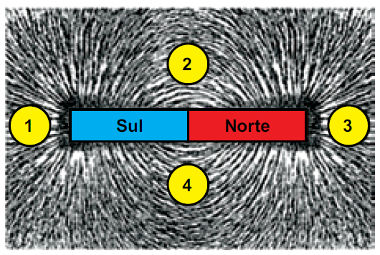
\includegraphics[width = 0.4\textwidth]{ex_2_unesp.jpg}
            \end{figure}
            Desconsiderando o campo magnético terrestre e considerando que a agulha magnética de cada bússola seja representada por uma seta que se orienta na mesma direção e no mesmo sentido do vetor campo magnético associado ao ponto em que ela foi colocada, assinale a alternativa que indica, correta e respectivamente, as configurações das agulhas das bússolas 1, 2, 3 e 4 na situação descrita.
            \pagebreak
            
            \begin{enumerate}
                \item 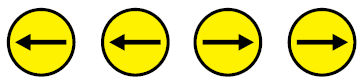
\includegraphics[width=0.2\textwidth]{letra-a.jpg} 
                \item 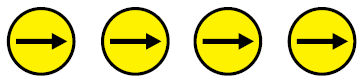
\includegraphics[width=0.2\textwidth]{2-letra-b.jpg}
                \item 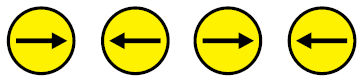
\includegraphics[width=0.2\textwidth]{2-letra-c.jpg}
                \item 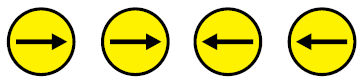
\includegraphics[width=0.2\textwidth]{2-letra-d.jpg}
                \item 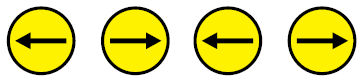
\includegraphics[width=0.2\textwidth]{2-letra-e.jpg}
            \end{enumerate}
            
            \item \textbf{(IFSP)} - Um professor de Física mostra aos seus alunos 3 barras de metal AB, CD e EF que podem ou não estar magnetizadas. Com elas, faz três experiências que consistem em aproximá-las e observar o efeito de atração e/ou repulsão, registrando-o na tabela a seguir.
            \begin{figure}[h]
                \centering
                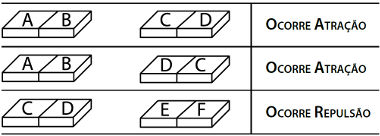
\includegraphics[width=0.4\textwidth]{ex_3_ifsp.jpg}
            \end{figure}
            
            Após o experimento e admitindo que cada letra pode corresponder a um único polo magnético, seus alunos concluíram que:
            
            \begin{enumerate}
                \item Somente a barra CD é ímã. 
                \item Somente as barras CD e EF são ímãs.
                \item Somente as barras AB e EF são ímãs.
                \item Somente as barras AB e CD são ímãs.
                \item AB, CD e EF são ímãs.
            \end{enumerate}
            
            \item Leia as afirmações a seguir sobre imãs:
            
            \begin{enumerate}
                \begin{enumerate}
                    \item As linhas de campo magnético dentro de um ímã de barra dirigem-se de sul para norte.
                    \item Não existe monopolo magnético.
                    \item Os materiais diamagnéticos (materiais como a água) são fracamente atraídos por ímãs.
                    \item Ferro, cobalto e alumínio são exemplos de materiais ferromagnéticos, que são fortemente atraídos por ímãs.
                \end{enumerate}
            \end{enumerate}
            
            Quais itens acima estão corretos?
            
            \item
            A imagem a seguir mostra um ímã permanente que foi quebrado ao meio.
            
            \begin{figure}[h]
                \centering
                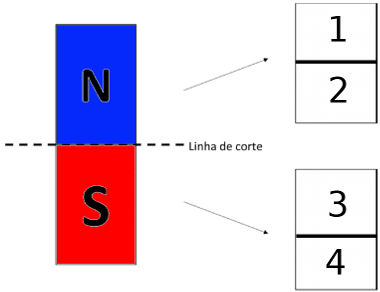
\includegraphics[width=0.4\textwidth]{ex_5.jpg}
            \end{figure}
            
            Sabendo que N e S representam, respectivamente, os polos norte e sul do ímã permanente, determine a polaridade dos pontos 1, 2, 3 e 4.
            
            \begin{enumerate}
                \item 1-sul, 2-norte, 3-sul e 4-sul. 
                \item 1-norte, 2-sul, 3-sul e 4-norte.
                \item 1-norte, 2-sul, 3-norte e 4 -sul.
                \item 1-sul, 2-sul, 3-norte e 4-norte.
                \item 1-norte, 2-sul, 3-norte e 4-norte.
            \end{enumerate}
        \end{enumerate}
        
    \end{itemize}
    \pagebreak
    \section*{GABARITO}
    \begin{itemize}
        \item \textbf{Imãs}
    \begin{enumerate}
        \item
        \begin{enumerate}
            \item F - O polo norte de imã é o positivo, enquanto o polo sul é o negativo.
            \item F - Ao quebrarmos um imã, as duas partes se tornam 2 imãs em que cada imã tem um polo norte e um polo sul.
            \item V - Lei de atração e repulsão dos polos.
            \item F - Um material é dito ferromagnético se ele é atraído por um imã, exemplo: ferro.
            \item F - materiais orgânicos, em sua grande maioria, são compostos de ametais, como o oxigênio, e somente os metais são atraídos por imã.
            \item V - Imãs artificiais são construídos a partir de processos como esfriamento do material a temperaturas muito baixas (algo entorno de $-100^{\circ}C$, dependendo do material, a temperatura pode ser menor). A temperaturas altas, a imantação se perde por causa da agitação das moléculas. Essas outras justificativas (contato e oxidação) "sujam" o imã com outros compostos e isso faz decrescer a imantação.
            \item V - O HD é basicamente uma fita magnética enrolada, em que os elétrons são colocados lá de forma que codificam a informação. Uma vez passando um imã na parede do HD, isso bagunça esses elétrons lá dentro da fita, perdendo a informação que eles guardavam. Após passar um imã no HD, o HD é perdido de vez (não há como reutilizá-lo). Por essa razão, não é recomendável colocar imãs de geladeiras (por mais que eles sejam fracos) nas paredes de um computador, pois pode estragar o HD.
        \end{enumerate}
        \item (c)
        \item (b)
        \item i e ii. A iii está errada, pois materiais diamagnéticos são repelidos por imãs e iv está errada, pois alumínio não é atraído por imãs.
        \item (c)
    \end{enumerate}
   \end{itemize}
\end{document}
